% \subsection{Effect of Type of Wealth on Inequality Measure} \label{wealth & gini}
\subsection{Impact of Wealth Type on Knowledge Inequality} \label{wealth & gini}

% \begin{center}
    \small
    \begin{threeparttable}
    \caption{Gini Bag-Set}
    \label{tab:gini bag-set}
    \begin{tabular}{c c c} 
    
    \toprule
        Class Name & Gini Bag & Gini Set \\ [0.5ex] 
    \midrule
        Historical painting & 0.22 & 0.14 \\
        University & 0.44 & 0.41 \\
        Sci-fi book & 0.32 & 0.22 \\
        Memorial & 0.22 & 0.18 \\
        American researcher & 0.33 & 0.31 \\
        American singer & 0.40 & 0.39 \\
        Badminton player & 0.29 & 0.14 \\
        Computer scientist & 0.41 & 0.37 \\
        [1ex]
    \bottomrule
    \end{tabular}
    \begin{tablenotes}
        \footnotesize
        This table shows the measures of gini coefficient of knowledge wealth based on the (non-)uniqueness of individual properties of 8 Wikidata classes
    \end{tablenotes}
    \end{threeparttable}
\end{center}
% \begin{center}
    \small
    \begin{threeparttable}
    \caption{Gini Object-Literal-ID}
    \label{tab:gini proptype}
    \begin{tabular}{c c c c} 
    
    \toprule
        Class Name & Gini Object & Gini Literal & Gini ID \\ [0.5ex] 
    \midrule
        American researcher & 0.26 & 0.50 & 0.50 \\
        American singer & 0.29 & 0.50 & 0.53 \\
        Badminton player & 0.30 & 0.36 & 0.60 \\
        Computer scientist & 0.36 & 0.54 & 0.56 \\
        Historical painting & 0.25 & 0.27 & 0.44 \\
        Memorial & 0.20 & 0.30 & 0.40 \\
        Sci-fi book & 0.35 & 0.34 & 0.42 \\
        University & 0.40 & 0.49 & 0.53 \\
        [1ex]
    \bottomrule
    \end{tabular}
    \begin{tablenotes}
        \footnotesize
        This table shows the measures of gini coefficient of knowledge wealth based on types of property of 8 Wikidata classes
    \end{tablenotes}
    \end{threeparttable}
\end{center}
% \begin{center}
    \small
    \begin{threeparttable}
    \caption{Gini Outgoing-Incoming}
    \label{tab:gini outgoing-incoming}
    \begin{tabular}{c c c} 
    
    \toprule
        Class Name & Gini Outgoing & Gini Incoming \\ [0.5ex] 
    \midrule
        Historical painting & 0.22 & 0.86 \\
        University & 0.44 & 0.91 \\
        Sci-fi book & 0.32 & 0.82 \\
        Memorial & 0.22 & 0.99 \\
        American researcher & 0.33 & 0.77 \\
        American singer & 0.40 & 0.82 \\
        Badminton player & 0.29 & 0.68 \\
        Computer scientist & 0.41 & 0.81 \\
        [1ex]
    \bottomrule
    \end{tabular}
    \begin{tablenotes}
        \footnotesize
        This table shows the measures of gini coefficient of knowledge wealth based on the direction of link of 8 Wikidata classes
    \end{tablenotes}
    \end{threeparttable}
\end{center}

\begin{table}[!htbp]
    \centering
    \renewcommand{\arraystretch}{1.3}
    \begin{tabular}{|l p{12cm}|} 
        \hline
        \multicolumn{2}{|l|}{\textbf{Impact of Wealth Type on Knowledge Inequality}} \\
        \hline
        \textbf{Insight 1:} & Wealth based on the bag of properties is always higher than that based on the set of properties, leading to higher value of Gini coefficient. \\
        \textbf{Insight 2:} & Wealth measured using incoming links shows significantly higher inequality than outgoing links. Lorenz curves confirm that very few entities have incoming links, while most have none. \\
        \textbf{Insight 3:} & In general, the order of Gini coefficient values from smallest to largest is: object properties, literal properties, and ID properties. \\
        \hline
    \end{tabular}
\end{table}

In this subchapter, analysis is done to see how each wealth type affects the level of knowledge inequality of Wikidata classes. There are 2 ways this is done--quantitatively using Gini coefficient and qualitatively using Lorenz curve. The analysis is performed on 8 Wikidata classes, in which 4 of them are human-related class while the other 4 are not.

\begin{center}
    \scriptsize
    \makebox[\linewidth]{
    \begin{threeparttable}
    \captionsetup{font=small}
    \caption{Knowledge Wealth Type on Gini Coefficient}
    \label{table:gini-coef}
    \begin{tabular}{c | c c | c c c | c c} 
    
    \toprule
        Class Name & \CellWithForceBreak{Gini \\ Bag} & \CellWithForceBreak{Gini \\ Set} & \CellWithForceBreak{Gini \\ Object} & \CellWithForceBreak{Gini \\ Pure Literal} & \CellWithForceBreak{Gini \\ ID} & \CellWithForceBreak{Gini \\ Outgoing} & \CellWithForceBreak{Gini \\ Incoming} \\ [0.5ex] 
    \midrule
        American researcher & 0.33 & 0.31 & 0.26 & *0.65 & 0.50 & 0.33 & 0.77 \\
        American singer & 0.40 & 0.39 & 0.29 & 0.36 & 0.53 & 0.40 & 0.82  \\
        Badminton player & 0.29 & 0.14 & 0.30 & *0.14 & 0.60 & 0.29 & 0.68 \\
        Computer scientist & 0.41 & 0.37 & 0.36 & *0.64 & 0.56 & 0.41 & 0.81 \\
        Historical painting & 0.23 & 0.15 & 0.25 & 0.26 & 0.45 & 0.23 & 0.87 \\
        Memorial & 0.22 & 0.19 & 0.20 & 0.31 & 0.41 & 0.22 & 0.99 \\
        Sci-fi book & 0.30 & 0.21 & 0.31 & 0.33 & 0.44 & 0.30 & 0.82 \\
        University & 0.44 & 0.41 & 0.39 & 0.49 & 0.53 & 0.44 & 0.91 \\
        [1ex]
    \bottomrule
    \end{tabular}
    \begin{tablenotes}
        \scriptsize
        \item{This table shows the comparison of Gini coefficient of 8 Wikidata classes}
    \end{tablenotes}
    \end{threeparttable}
    }
\end{center}

When looking at the notion of wealth using the characteristics of (non-)uniqueness of individual properties, it is intuitive that the measure of the bag of properties will always give higher (or at least, equal) amount of wealth compared to the measure of set. Set of property will have an upper bound of number of unique property, while the bag of properties does not have any upper bound. Moreover, using the bag of properties, a large number of triples having the same property may inflate the wealth substantially--though this is not necessarily a problem nor an advantage. This characteristics has a direct impact on inequality measure and it is well depicted on the value of Gini coefficient. From \autoref{table:gini-coef}, in all clasess, the Gini coefficient using the bag of properties is always higher than of set of properties.

% - object, literal, ID: object tends to have lower inequality
Using the notion of wealth by type of property, in general the smallest Gini coefficient value comes from wealth using object properties, followed by literal properties, with ID properties having the highest value. This condition holds for the four non-human classes that are being observed. However, there are anomalies in the human classes, as illustrated in \autoref{fig:gini-literal}.

\begin{figure}[!htbp]
    \centering
    % 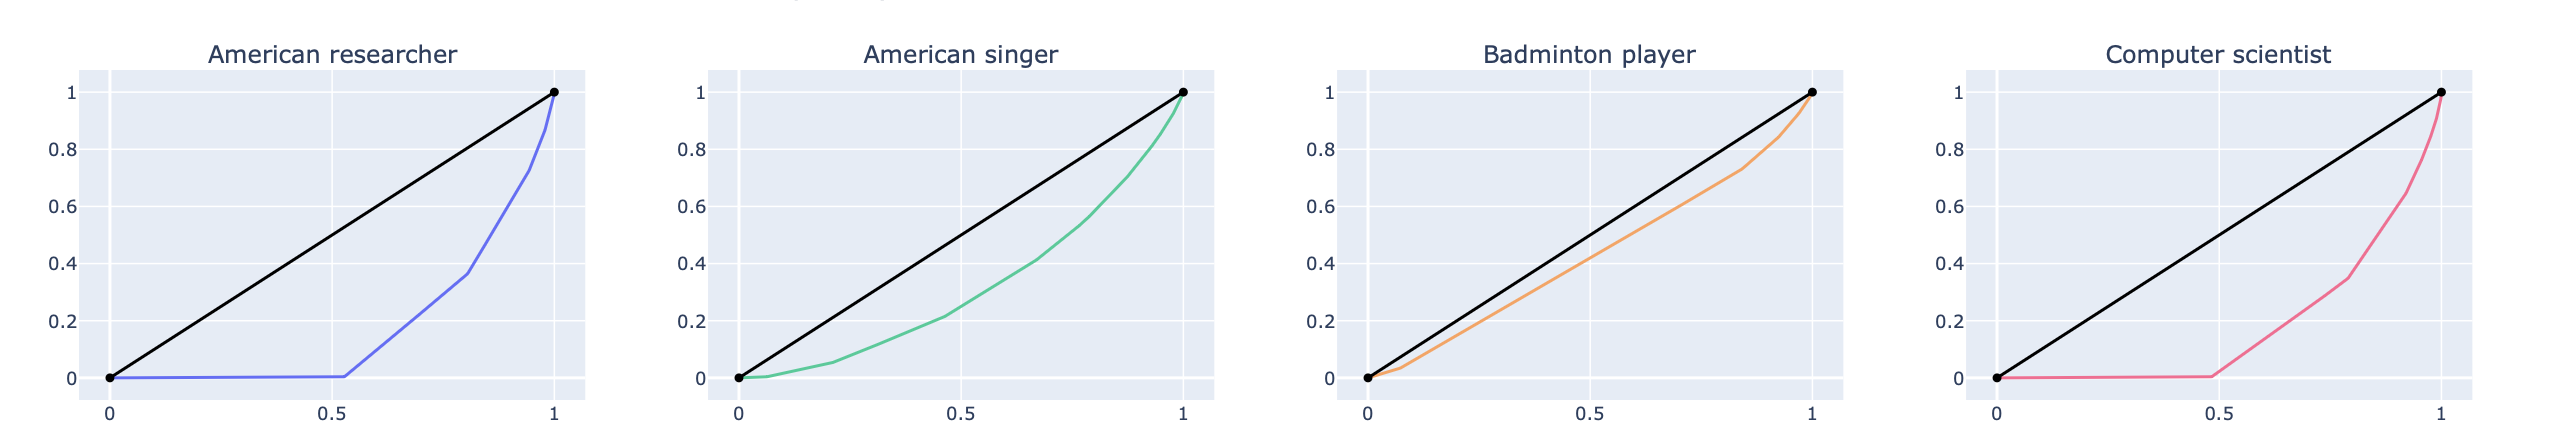
\includegraphics[scale=.5]{Gini - Pure Literal}
    \makebox[\textwidth][c]{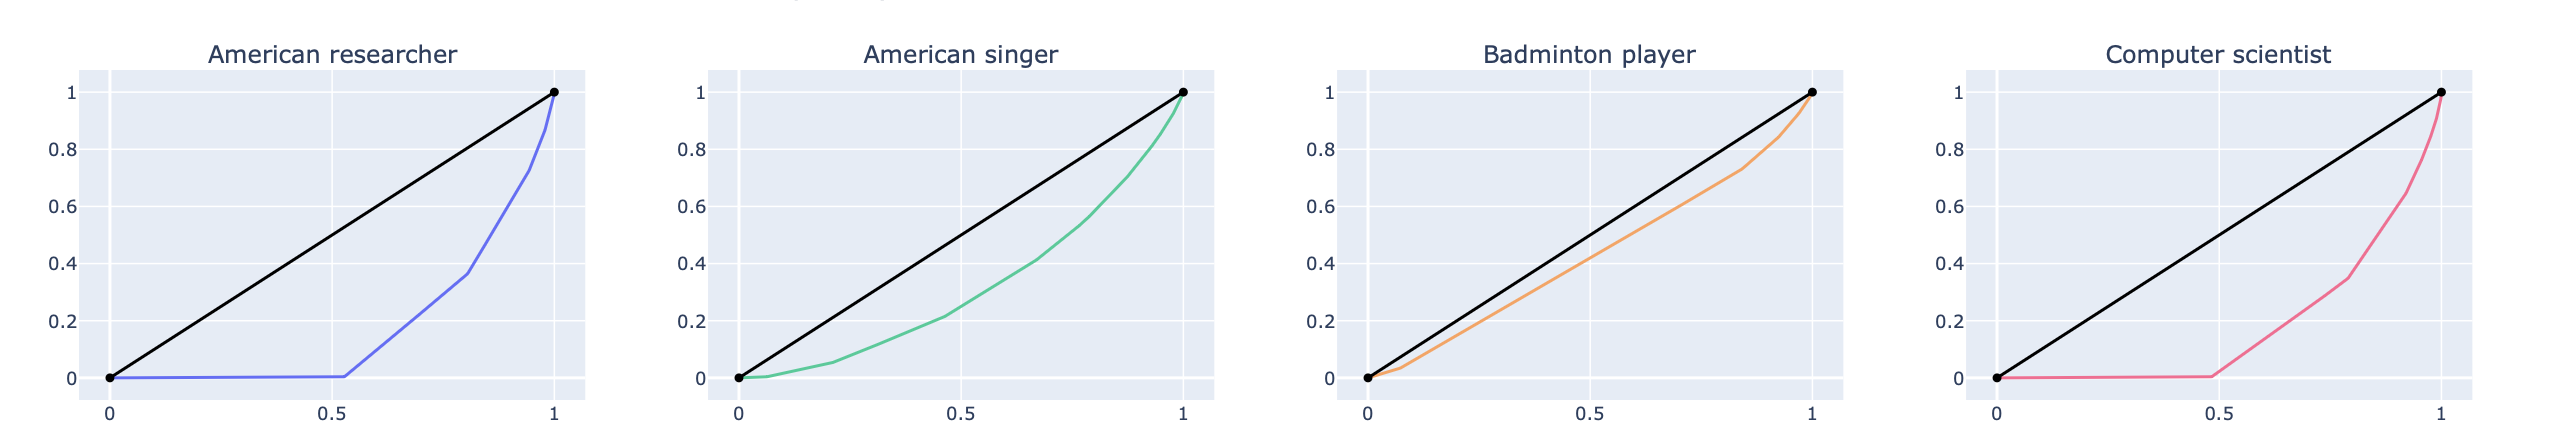
\includegraphics[width=1\textwidth]{Gini - Pure Literal}}%
    \caption{Lorenz curve of wealth using literal properties} \label{fig:gini-literal}
\end{figure}

In the classes of American researchers and computer scientists, the Gini coefficients for wealth using pure literal properties are significantly higher than those of other classes. This is due to approximately 50\% of the entities in these classes having 0 pure literal properties--not even basic human-related literal properties such as \textit{date of birth} (P569). For example, an American researcher \textit{John Heidemann} (Q29354581) has a total wealth of 61 (using the bag of properties) and is among the top 4\% entities in his class, yet this entity has 0 literal properties. In contrast, only 818 out of 16150 (just about 5\%) entities of American singer class have 0 literal properties. Moreover, an instance of American singer, \textit{Kris Allen} (Q216927), who also has a total wealth of 61 (using the bag of properties), has 6 literal properties.

Another anomaly is observed in the class of badminton player where the Gini coefficient for wealth using pure literal is significantly lower than that of other classes. Upon inspection, three main reasons for this anomaly were identified. First, there are no entities in this class with 0 literal properties; all entites have at least 1 literal. Second, the range of wealth in this class is smaller, with a minimum value of 1 and maximum value of 10, in comparison to the classes of American researcher, American singer, and computer scientist which all have a minimum value of 0 and maximum values of 16, 26, and 54, respectively. This smaller range means the difference between the poorest and richest entities in the class of badminton player is minimal, and a small wealth range generally leads to a low Gini coefficient because inequality is limited by the narrow spread of wealth. The third reason is the large number of entities in this class, which totals 25,402. With such a high population size, the wealth of each individual—whether the poorest, middle, or richest entity—contributes only a tiny fraction to the total wealth of the class. Combined with the small wealth range, this further reduces the inequality measure, resulting in a low Gini coefficient.

% - object: 
% - literal: analisis kenapa yang badminton beda sendiri (object > literal). perlu cek yang literal only tanpa ID (cek query vs hitung manual literala all - ID)
% - ID: ID itu kan menandakan apakah suatu entity terdaftar di suatu DB external lain. nah ini lebih sensitif terhadap popularitas entity. biasanya hanya entity yang populer banget yang  (aspek eksponensial, ketika dia populer dia terdaftar di banyak db dibandingkan yang medioker. ketika viral, dia kaya domina effect terdaftar lagi di yang lain2). semacam incoming link

% - outgoing, incoming: incoming shows very high Gini, this is because it is harder --> show the lorenz curve
Using the notion of wealth by the direction of the link, the Gini coefficient when using incoming link is always higher than using outgoing link. By inspecting the Lorenz curve, we can see that most entities do not have any incoming link, and only the small percentage of entites has some incoming link. \autoref{fig:gini-outgoing&incoming} shows the comparison of Lorenz curve of knowledge wealth based on the direction of the link from 3 Wikidata classes. The difference between the two is very significant, because in \autoref{fig:gini-outgoing} the Lorenz curves are closer to the perfect equality line, meanwhile in \autoref{fig:gini-incoming} the diagonal and the Lorenz curve almost form a right triangle which is very close to maximum inequality.

% add to discussion 
% - Wikidata = entity-centric knowledge graph, dimana bentuknya (s,p,o) dengan s sebagai subject of interest. jadi memang expected bahwa outgoing banyak 
% sedangkan incoming mostly justru 0.
% - sedrastis ini perbedaan incoming vs outgoing. incoming link is underestimated. given o, what is the (s, p)
% - kasih contoh: 2 entitas yang secara outgoing mirip, tapi incoming-nya jomplang (1 kaya 1 miskin)

\begin{figure}[!htbp]
    \centering 
    \subfloat[Lorenz curve of wealth using outgoing link
    \label{fig:gini-outgoing}]{%
      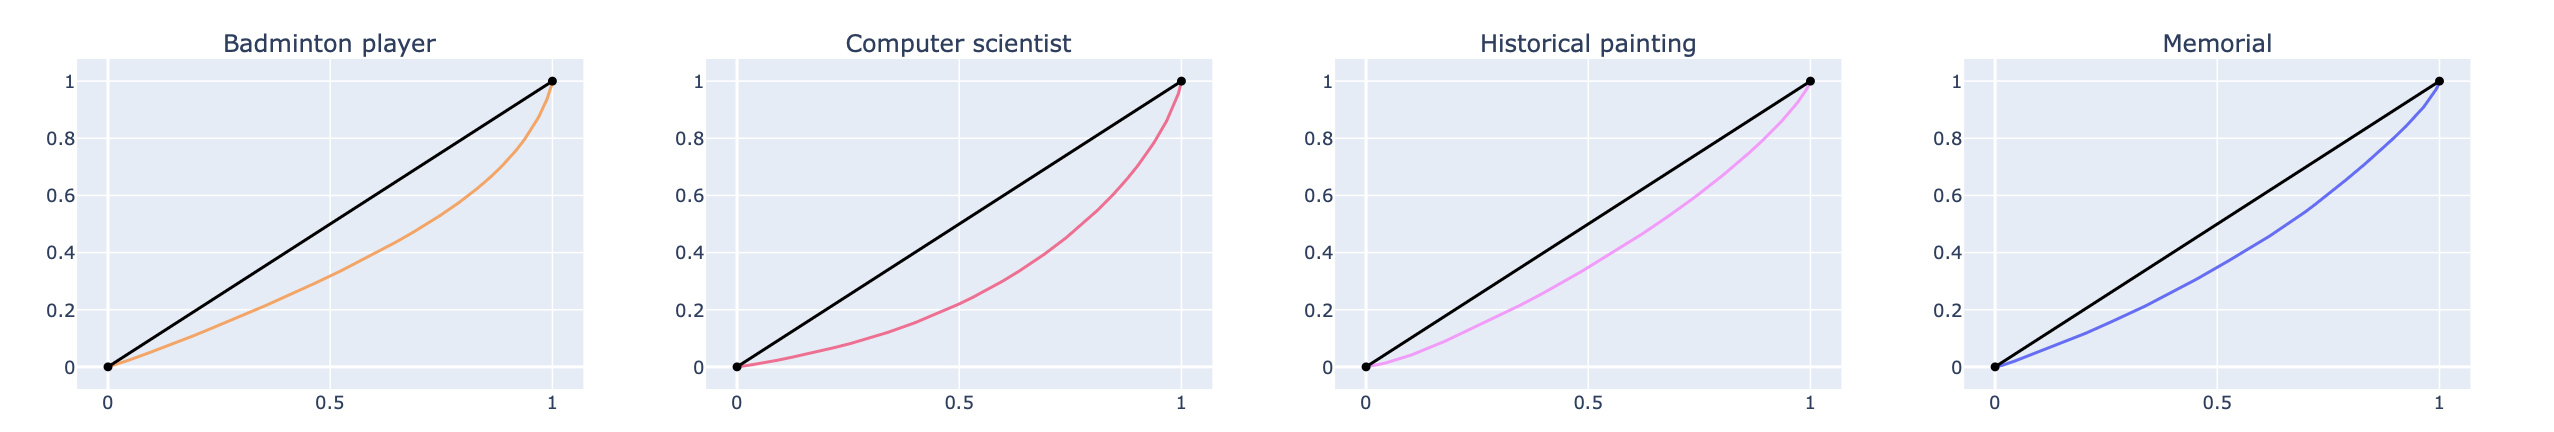
\includegraphics[clip,width=1.0\columnwidth]{Gini - Outgoing}%
    }
    
    \subfloat[Lorenz curve of wealth using incoming link\label{fig:gini-incoming}]{%
      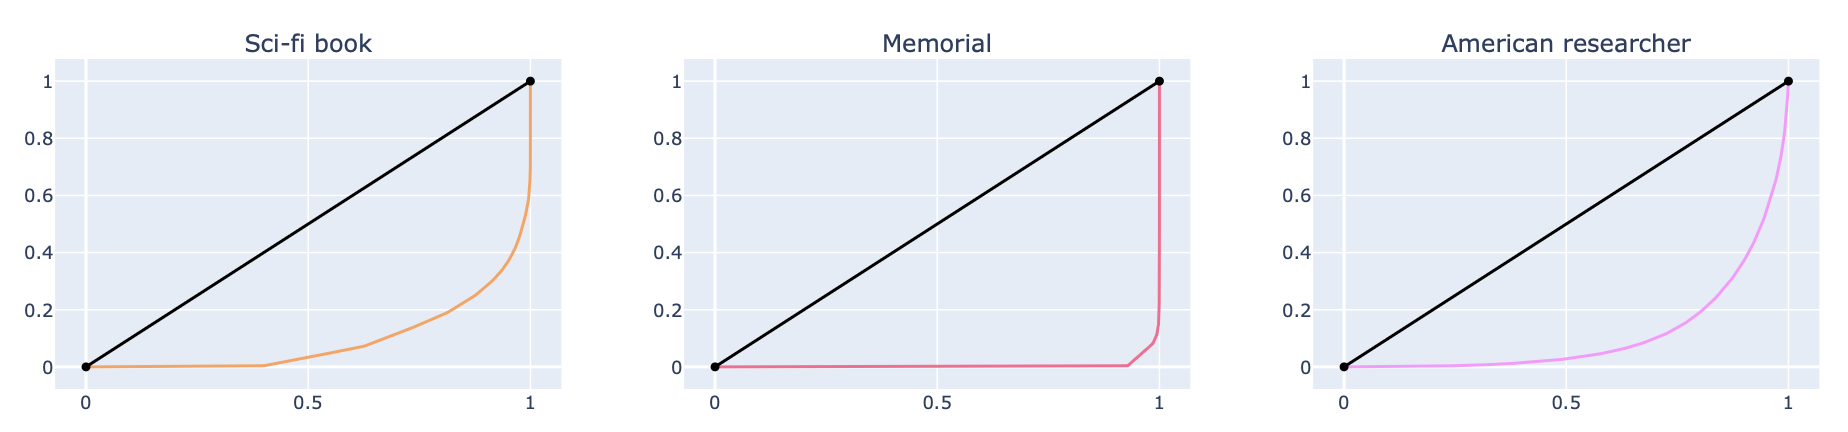
\includegraphics[clip,width=1.0\columnwidth]{Gini - Incoming.png}%
    }
    
    \caption{Comparison of Lorenz curve of wealth based on the direction of link} \label{fig:gini-outgoing&incoming}
    
\end{figure}